\section{Auswertung}
\label{sec:Auswertung}

\subsection{Messwerte}
\begin{table}[H]
    \centering
    \caption{Messwerte der vier Peaks zur Programmeinstellung.}
    \label{tab:10}
    \begin{tblr}{
            colspec = {S S S S S S},
            row{1} = {guard, mode = math},
        }
        \toprule
        \text{Peak}& \text{Laufzeit} / \unit{\micro\second}\\
        \midrule
        1  & 3.2\\
        2  & 30.0\\
        3  & 59.9\\
        4  & 89.4\\
        \bottomrule 
    \end{tblr}
\end{table}

\begin{table}[H]
    \centering
    \caption{Messwerte der Periodendauer.}
    \label{tab:11}
    \begin{tblr}{
            colspec = {S S S S S S},
            row{1} = {guard, mode = math},
        }
        \toprule
        \text{Periodendauer}/\unit{\micro\second}\\
        \midrule
        0.5\\
        0.6\\
        0.7\\
        0.5\\
        0.7\\
        0.7\\
        \bottomrule 
    \end{tblr}
\end{table}

\begin{table}[H]
    \centering
    \caption{Höhen der jewailigen zylinder sowie Laufzeiten zu den Grenzflächen.}
    \label{tab:12}
    \begin{tblr}{
            colspec = {S S S S S S},
            row{1} = {guard, mode = math},
        }
        \toprule
        \text{Zylinder}&\text{Laufzeit Acryl}/\unit{\micro\second} & \text{Laufzeit Alu}/\unit{\micro\second} & \text{Höhe Acryl}/\unit{\centi\meter}& \text{Höhe Alu}/\unit{\centi\meter}\\
        \midrule
        1 &  85.7  &  37.3  &  12.07+-0.01  & 12.35+-0.01\\
        2 &  73.2  &  33.9  &  10.22+-0.01  & 11.51+-0.01\\
        3 &  56.7  &  25    &  8.06 +-0.01  & 8.12 +-0.01\\
        4 &  43.2  &  19.1  &  6.17 +-0.01  & 6.22 +-0.01\\
        5 &  36.7  &  16.3  &  5.30 +-0.01  & 5.32 +-0.01\\
        6 &  27.5  &  12.2  &  4.03 +-0.01  & 4.01 +-0.01\\
        7 &  20.7  &  9.4   &  3.12 +-0.01  & 3.12 +-0.01\\
        8 &  65.9  &  16.5  &  9.33 +-0.01  & 9.33 +-0.01\\
        \bottomrule 
    \end{tblr}
\end{table}

\begin{table}[H]
    \centering
    \caption{Messwerte der Amplituden mit zwei verschiedenen Sonden.}
    \label{tab:13}
    \begin{tblr}{
            colspec = {S S S S S S},
            row{1} = {guard, mode = math},
        }
        \toprule
        \text{Zylinder}&A_{einf,2\unit{\mega\hertz}}\text{Acryl}/\unit{\micro\second} & A_{ref,2\unit{\mega\hertz}}\text{Acryl}/\unit{\micro\second} &A_{einf,1\unit{\mega\hertz}}\text{Acryl}/\unit{\micro\second} &A_{ref,1\unit{\mega\hertz}}\text{Acryl}/\unit{\micro\second}\\
        \midrule
        1 &  1.244 &  0.647 &  0.727  & 0.536\\
        2 &  1.244 &  0.62  &  0.727  & 0.609\\   
        3 &  1.244 &  0.385 &  0.727  & 0.617\\
        4 &  1.244 &  0.62  &  0.727  & 0.470\\
        5 &  1.244 &  0.604 &  0.727  & 0.470\\
        6 &  1.244 &  0.659 &  0.727  & 0.505\\
        7 &  1.244 &  0.724 &  0.727  & 0.393\\
        8 &  1.244 &  0.602 &  0.727  & 0.386\\
        \bottomrule 
    \end{tblr}
\end{table}


\begin{table}[H]
    \centering
    \caption{Laufzeiten zur Wasseroberfläche für verschiedene Füllmengen.}
    \label{tab:14}
    \begin{tblr}{
            colspec = {S S S S S S},
            row{1} = {guard, mode = math},
        }
        \toprule
        \text{Wassermenge} / \unit{\milli\liter} & \text{Laufzeit} / \unit{\micro\second}\\
        \midrule
        50 +-1& 19.2\\
        60 +-1& 22.2\\
        70 +-1& 24.2\\
        80 +-1& 26.7\\
        90 +-1& 29\\
        100+-1& 31.3\\
        110+-1& 33.6\\
        120+-1& 35.7\\
        130+-1& 38.2\\
        140+-1& 40.3\\
        150+-1& 42.7\\
        160+-1& 44.9\\
        170+-1& 47.2\\
        180+-1& 49.9\\
        190+-1& 52.4\\
        200+-1& 55.4\\
        \bottomrule 
    \end{tblr}
\end{table}

\subsection{Programm und Geräteeinstellungen}
Um die Funktionsweise des Programms zu verstehen wurden am Anfang 
zuerst vier $x$-Werte von Peaks (\autoref{fig:10} sowie Werte in \autoref{tab:10})
bei der Durchschallung eines Acrylblockes mit der $2 \unit{\mega\hertz}$ Sonde
aufgenommen. Diese entstehen durch Reflexion an der Grenzfläche bei Eintritt in
das Acryl und bei Austritt sowie auch weitere Male mit geschwächter Ampilitude.
Um trotzdem die hinteren Peaks erkennbar zu machen wurde die Verstärkung,
welche unten im Bild zu erkennen ist, eingeschaltet.
\begin{figure}[H]
    \centering
    \caption{Peaks der Grenzflächenreflexion.}
    \label{fig:10}
    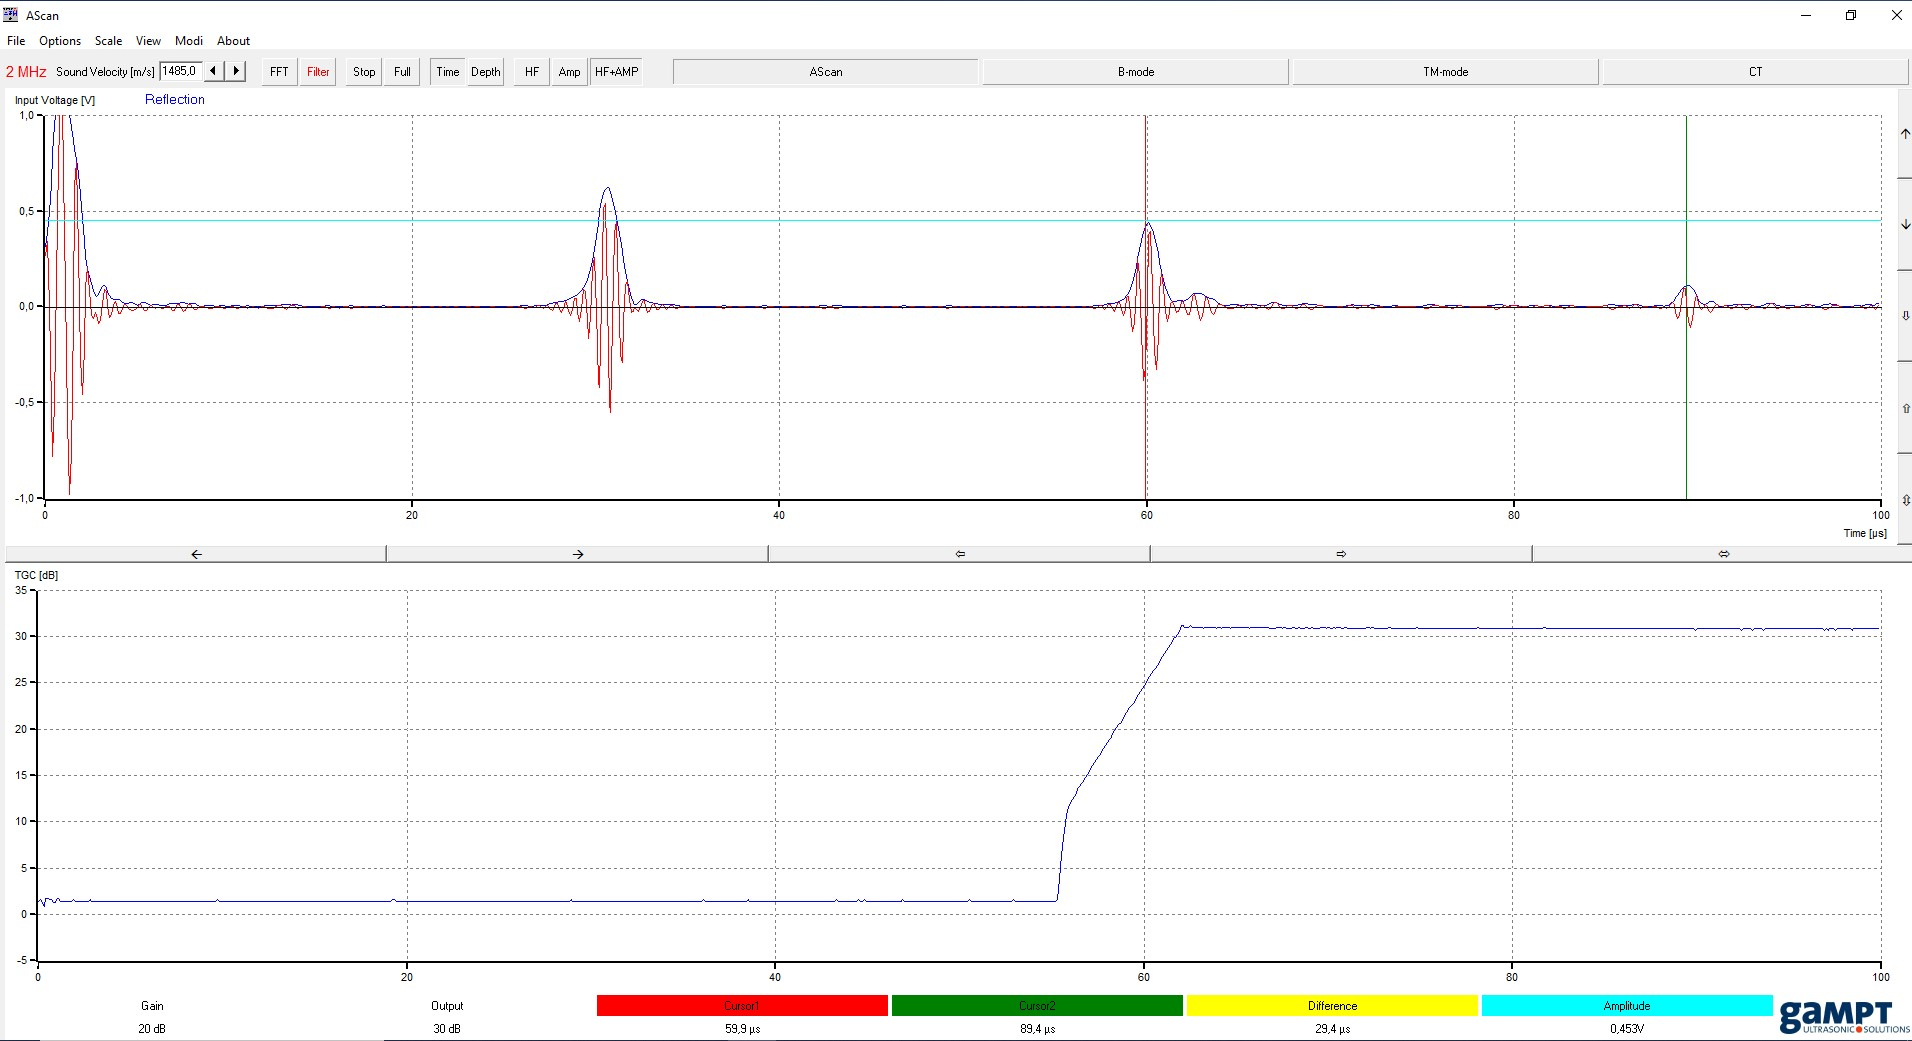
\includegraphics[width=\textwidth]{bilder/ssprogramm.jpg}
\end{figure}
\noindent Des Weiteren wurden der Abbildung mehrere Periodendauern $T$ entnommen, indem 
der Zeitabstand zwischen Anfang und Ende einer ganzen Schwingugsperiode 
gemessen wurde. Diese Werte aus \autoref{tab:11} wurden gemittelt, das
ergibt eine mittlere Periodendauer von 
\begin{equation}
   T = \qty{0.61(0.04)}{\micro\second}.
\end{equation}
Unter Annahme der später bestimmten Schallgeschwindigkeit in Acryl von
$c_\text{Acryl} = \qty{2744(14)}{\meter\per\second}$ ergibt sich eine
durchschnittliche Wellenlänge von
\begin{equation}
   \lambda = \qty{1.69(0.11)}{\milli\meter}.
\end{equation}

\subsection{Schallgeschwindigkeit in Acryl und Aluminium}
Die Schallgeschwindigkeiten in den verschiedenen Medien werden ermittelt,
indem die Höhe der Zylinder gegen die halbe Laufzeitdifferenz des Ultraschalls 
zwischen Anfangs- und Endgrenzfläche aufgetragen wird. Wird eine Ausgleichsgerade
der Form $y = m \cdot x + b$ an die Messwerte gefittet, kann die Schallgeschwindigkeit 
duch den Steigungsparameter $m$ bestimmt werden. Die Messwerte der Höhen sowie
die Laufzeiten befinden sich für Aluminium und Messing in \autoref{tab:12} 
und die graphischen Darstellungen für Acryl in \autoref{fig:11} und für Aluminium
in \autoref{tab:12}.
\begin{figure}[H]
    \centering
    \caption{Messwerte und Regression zur Ermittlung der Schallgeschwindigkeit in Acryl.}
    \label{fig:11}
    \includegraphics{build/schallgeschwindigkeit_acryl.pdf}
\end{figure}
\noindent Die Parameter der Ausgleichsrechnung ergeben sich zu 
\begin{align*}
    a &= \qty{2744(14)}{\meter\per\second}\\
    b &= \qty{0.002(0.0004)}{\meter}.
\end{align*}
Somit ergibt sich eine Schallgeschwindigkeit in Acryl von 
\begin{equation}
    c_\text{Acryl} = \qty{2744(14)}{\meter\per\second}.
\end{equation}

\begin{figure}[H]
    \centering
    \caption{Messwerte und Regression zur Ermittlung der Schallgeschwindigkeit in Aluminium.}
    \label{fig:12}
    \includegraphics{build/schallgeschwindigkeit_alu.pdf}
\end{figure}
\noindent Die Parameter der Ausgleichsrechnung ergeben sich zu 
\begin{align*}
    a &= \qty{6213(1107)}{\meter\per\second}\\
    b &= \qty{0.0091(0.012)}{\meter}.
\end{align*}
Somit ergibt sich eine Schallgeschwindigkeit in Acryl zu
\begin{equation}
    c_\text{Aluminium} = \qty{6213(1107)}{\meter\per\second}.
\end{equation}

\subsection{Dämpfungsfaktor}
Um den Dämpfungsfaktor der Schwingungsamplitude zu ermitteln, werden die
Amplituden der reflektierten Schwingungen an den Grenzflächen bei verschiedenen
Abständen des Ultraschalls betrachtet. Die Amplituden aus \autoref{tab:13} werden
in \autoref{fig:13} (2$\unit{\mega\hertz}$ Sonde) sowie in \autoref{fig:14} 
(1$\unit{\mega\hertz}$ Sonde) gegen die Abstände der jeweiligen Grenzfläche 
(Höhen der Zylinder) aufgetragen und dann eine Regression der Form 
$y = m \cdot x + b$  durchgeführt. In \autoref{fig:131} und \autoref{fig:141} sind
die fits der ursprünglichen Messwerte aufgetragen, jedoch fallen einige
Messwerte so weit aus dem Muster, dass in \autoref{fig:13} der Messwert 3 rausgenommen wurde und in \autoref{fig:14} die Werte 1,2 und 7.
Somit ergeben sich deutlich sinnvollere und genauere Dämpfungsfaktoren.
 
\begin{figure}[H]
    \centering
    \caption{Messwerte und Regression der Amplituden Mit der 2 $\unit{\mega\hertz}$ Sonde ohne Wert 3.}
    \label{fig:13}
    \includegraphics{build/amplituden_alu2mhzbearbeitet.pdf}
\end{figure}
Die Parameter der Ausgleichsrechnung ergeben sich zu 
\begin{align*}
    a &= \qty{-0.82(0.7)}{1 \per\meter}\\
    b &= \qty{0.60(0.05)}{}
\end{align*}
Somit ergibt sich ein Dämpfungsfaktor von 
\begin{equation}
    d_{2\unit{\mega\hertz},angepasst} = \qty{0.82(0.7)}{1 \per\meter}.
\end{equation}

\begin{figure}[H]
    \centering
    \caption{Messwerte und regression der Amplituden Mit der 1 $\unit{\mega\hertz}$ Sonde ohne die Werte 1,2 und 7}
    \label{fig:14}
    \includegraphics{build/amplituden_alu1mhzbearbeitet.pdf}
\end{figure}
\noindent Die Parameter der Ausgleichsrechnung ergeben sich zu 
\begin{align*}
    a &= \qty{-1.6(4.4)}{1 \per\meter}\\
    b &= \qty{-0.29(0.30)}{\meter}.
\end{align*}
Somit ergibt sich ein Dämpfungsfaktor von 
\begin{equation}
    d_{1 \unit{\mega\hertz},angepasst} = \qty{1.6(4.4)}{1 \per\meter}.
\end{equation}

\subsubsection{Ursprüngliche Messwerte}
\begin{figure}[H]
    \centering
    \caption{Messwerte und Regression der Amplituden Mit der 2 $\unit{\mega\hertz}$ Sonde.}
    \label{fig:131}
    \includegraphics{build/amplituden_alu2mhz.pdf}
\end{figure}
\noindent Die Parameter der Ausgleichsrechnung ergeben sich zu 
\begin{align*}
    a &= \qty{-1.47(2.37)}{1 \per\meter}\\
    b &= \qty{-0.62(0.19)}{\meter}.
\end{align*}
Somit ergibt sich ein Dämpfungsfaktor von 
\begin{equation}
    d_{2 \unit{\mega\hertz}} = \qty{1.47(2.37)}{1 \per\meter}.
\end{equation}

\begin{figure}[H]
    \centering
    \caption{Messwerte und Regression der Amplituden Mit der 1 $\unit{\mega\hertz}$ Sonde }
    \label{fig:141}
    \includegraphics{build/amplituden_alu1mhz.pdf}
\end{figure}
\noindent Die in \autoref{fig:141} dargestellte Regression
der ursprünglichen Messdaten ergeben eine positive Steigung. Dieses Ergebnis
ist physikalisch nicht plausibel, da es einer Verstärkung der Schwingungen
durch das Material entsprechen würde.
Die Daten zu dem Graphen wären:
\begin{align*}
    a &= \qty{2.46(2.06)}{1 \per\meter}\\
    b &= \qty{-0.57(0.16)}{\meter},
\end{align*}
sodass sich ein Dämpfungsfaktor von 
\begin{equation}
    d_{1 \unit{\mega\hertz}} = \qty{-2.46 \pm 2.06}{\per\meter}
\end{equation}
ergibt.

\subsection{Kallibrierkurve}
Es wird davon ausgegangen, dass der Füllstand eines Erlenmeyer-Kolbens durch
eine Funktion dritten Grades genähert werden kann. Es werden die Messwerte 
aus \autoref{tab:14} an eine Funktion der Form $y = a \cdot x^2 + b \cdot x + c $ gefittet 
um die Parameter der Füllstandsfunktion zu bestimmen. 
\begin{figure}[H]
    \centering
    \caption{Messwerte und Regression des Füllstandes gegen die Laufzeit.}
    \label{fig:15}
    \includegraphics{build/fuellstand.pdf}
\end{figure}

\noindent Mit den Parametern 
\begin{align}
    a &= \qty{0.000(0.000)}{\frac{\milli\liter}{\micro\second^2}}, \\
    b &= \qty{0.217(0.010)}{\frac{\milli\liter}{\micro\second}}, \\
    c &= \qty{8.694(0.552)}{\milli\liter}
\end{align}
der Regression ergibt sich die Füllstandsfunktion zu 
\begin{equation}
    u_\text{füllstand}(x) = 0 \cdot x^2 + 0.21 \cdot x + 8.69.
\end{equation}

